\section{Results: Kyber in Comparison with Non-PQE Messaging Applications}

This section summarizes the results of the comparisons of Kyber with non-PQE messaging applications. This comparison considers the security analysis, implementation, and performance aspects described in previous sections.

\subsection{Resistance to a Quantum Adversary}

The first result is that Kyber stays safe in the environment where quantum computing is possible~\cite{shor,grover}. At the same time, non-PQE applications only use classical algorithms for generating keys, such as X25519~\cite{rfc7748}. When a quantum computer becomes sufficiently big, Shor’s algorithm breaks the discrete logarithm used in these exchanges and allows an adversary to calculate session keys based on captured handshakes.

To solve this problem, Kyber uses two approaches at once. The session key of Kyber is calculated using both X25519 and ML-KEM-768~\cite{rfc7748,fips203} algorithms. An adversary has to break both of them to obtain the session key. Figure \ref{fig:result_comparison} shows this difference. An exchange that can be broken by a classical adversary cannot provide any resistance to a quantum adversary. At the same time, a hybrid approach implemented in Kyber retains its safety against both types of adversaries.

Figure depicts a sample comparison of the possible security levels that can be reached for protection against classical and quantum attackers. It compares a purely classical key agreement mechanism based on X25519 (RFC 7748) to a mixed one which is a combination of X25519 and ML-KEM-768 (Kyber, mixed mechanism, as defined in FIPS 203). The axes represent the adversary type (x-axis) and security (bits) (y-axis). The markers correspond to the security levels: 64, 128, and 192 bits. Figure also identifies the types of attacks on the mechanism through the use of shading: classical attack on the left part and quantum attack on the right part.

\begin{figure}[htbp]
\centering
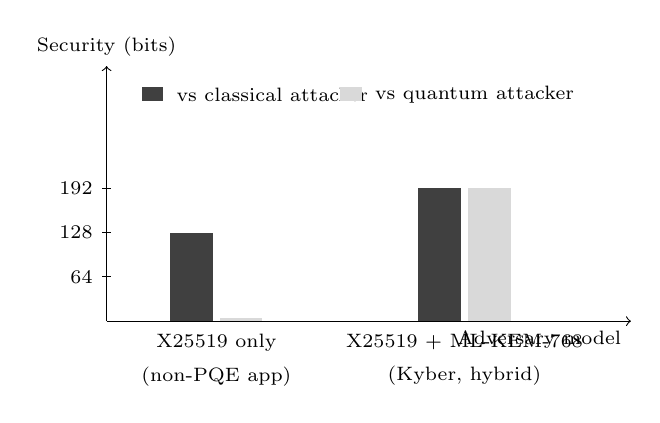
\begin{tikzpicture}[scale=0.9]
    \draw[->] (0,0) -- (7.4,0) node[below left] {\scriptsize Adversary model};
    \draw[->] (0,0) -- (0,3.6) node[above] {\scriptsize Security (bits)};
    \foreach \y/\l in {0.625/64, 1.25/128, 1.875/192} {
        \draw (0.06,\y) -- (-0.06,\y) node[left] {\scriptsize \l};
    }
    \fill[black!75] (0.9,0) rectangle (1.5,1.25);
    \fill[black!15] (1.6,0) rectangle (2.2,0.04);
    \fill[black!75] (4.4,0) rectangle (5.0,1.875);
    \fill[black!15] (5.1,0) rectangle (5.7,1.875);
    \node[align=center] at (1.55,-0.55) {\scriptsize X25519 only\\ \scriptsize (non-PQE app)};
    \node[align=center] at (5.05,-0.55) {\scriptsize X25519 + ML-KEM-768\\ \scriptsize (Kyber, hybrid)};
    \fill[black!75] (0.5,3.1) rectangle (0.8,3.3);
    \node[right] at (0.85,3.2) {\scriptsize vs classical attacker};
    \fill[black!15] (3.3,3.1) rectangle (3.6,3.3);
    \node[right] at (3.65,3.2) {\scriptsize vs quantum attacker};
\end{tikzpicture}
\caption{Illustrative comparison of effective security against classical and quantum attackers: a classical-only exchange (X25519~\cite{rfc7748}) versus the hybrid exchange used by Kyber (X25519 + ML-KEM-768~\cite{fips203}).}
\label{fig:result_comparison}
\end{figure}

\subsubsection{Harvest-Now-Decrypt-Later Security}

The harvest-now-decrypt-later situation makes this possible in reality right now, not in some distant future~\cite{bsi_hybrid}. An attacker could intercept the ciphertext traffic of a non-PQE application right now and only then use a quantum computer to decrypt it. Therefore, all the messages collected today, including their keys, identities, and history, may become readable after some time.

The Kyber algorithm prevents this attack. As the session key is derived in a hybrid exchange, the intercepted ciphertexts stay secure even if stored for a very long period. Thus, this provides an important advantage of Kyber over non-PQE apps in cases where the information needs to be secured for a long time, like personal, medical, or business data.

\subsubsection{Comparison With Deployed Post-Quantum Messengers}

Post-quantum protection is also provided in Signal PQXDH and Apple PQ3 messengers~\cite{pqxdh,pq3}, and Kyber uses a similar hybrid scheme. The difference is in the way these messengers are deployed: these messengers are proprietary and platform-specific software, while Kyber shows that the same level of protection can be achieved with a standard Flutter app using local keys storage and a simple relay server.

In normal usage, the cost of this protection is minimal. The hybrid exchange is done just once for each chat, and each message is still encrypted using AES-256-GCM~\cite{gcm} with the same overhead per message as for a non-PQE application. Just the key sizes grow~\cite{fips203}, but the keys are either stored on the device or transmitted as ciphertexts. Hybrid encryption schemes similar to this one have already been developed and adopted in TLS and VPN protocols~\cite{ietf_hybrid_tls,ietf_hybrid_ike}.

\subsection{Summary of Results}

\begin{itemize}
    \item \textbf{Quantum-resilience}: Kyber guarantees the secrecy of the session keys even under a quantum attacker's influence, unlike any other non-PQE app where there is a risk of key compromise~\cite{shor,fips203}.
    
    \item \textbf{Privacy in the long run}: Captured Kyber-enabled traffic cannot be decrypted retroactively~\cite{bsi_hybrid}.
    
    \item \textbf{Classical security properties}: The X25519 algorithm provides classical secure messaging properties that were previously studied~\cite{doubleratchet,rfc7748}.
    
    \item \textbf{Little extra computation}: The additional computational expense is required only once, at the start of a conversation, not for each new message~\cite{gcm}.
    
    \item \textbf{Practicality}: The developed solution is a working application able to run on an ordinary mobile device rather than a purely theoretical protocol~\cite{pqxdh,pq3}.
\end{itemize}

The problems inherent in the prototype are still present: metadata leaking from the relay, the problem of first-contact trust and the necessity of access control policies~\cite{dolev_yao}. Even so, the takeaway is simple: combining a classical exchange with a post-quantum one keeps Kyber's chats safe against attacks that would break a non-PQE app, while the app itself stays light enough for daily use on an ordinary phone.
